\section{The Model}
The proposed model aims at simulating the mobility of individuals in Milan that use the public transport services, exploring the consequences of shocks and interventions that can affect directly the transport network. Specifically, the elements that constitute the model are:
\begin{itemize}
    \item \textbf{The environment:} the public transport network of Milan, including metro, tram, bus and filobus lines.
    \item \textbf{The agents:} synthetic individuals, constituting the flow of passengers on ATM vehicles.
    \item \textbf{The time:} the simulation is based on data regarding an ordinary week day, from 5:00 a.m. to 1.00 a.m. of the next day and each step represents 1 minute (for a total of 1200 steps).
    \item \textbf{The rules:} agents, according to their schedules, move on the network, respecting the timetables and the availability in terms of capacity on the vehicles.
\end{itemize}
The idea of the model is to generate synthetic agents, place them on the graph representing the transport network of the city of Milan, and let them move around the city according to their schedules. Individuals interact with each others as they compete to get on the same vehicle, since vehicles have limited capacity. Moreover, they interact with the environment, since they choose the shortest path to their destinations, according to network-specific attributes (i.e. distance between stops, speeds of the vehicles, lines' timetables). 

\subsection{Data and manipulation}\label{sec3}
The model is based on different datasets describing the Milan's transport network and population. We distinguish between those needed to build the transport network and those used in the process of synthesizing the population and highlight the main steps of the manipulation process.\\ \\
The datasets used to build the network are the following:
\begin{enumerate}
    \item Two datasets \cite{site1, site5} from Comune di Milano's open data, containing the main features characterizing each route of the underground lines and  of the surface transit lines respectively: an id number, the mean of transport, the line, the terminal points and their geographical coordinates, the length and the number of stops. A line can have multiple routes, active in different time ranges.  
    \item Two datasets \cite{site2, site6} from Comune di Milano's open data, containing the AMAT\footnote{Agenzia Mobilità Ambiente e Territorio, an agency, present in the municipality of Milan, that provides services to support the municipal functions in the fields of planning, programming, management, monitoring and control relating to the development of the territory and greenery, urban planning, mobility and transport public \cite{site21}.} id, the line name and number, the geographical coordinates and the location of all the stops of the metro lines and of the surface transit lines respectively.
    \item Two datasets \cite{site3, site7} from Comune di Milano's open data, containing the sequence of stops for each route of the underground lines and of the surface transit lines respectively;
    \item Two datasets \cite{site4, site8} from Comune di Milano's open data, containing the starting time, the ending time, the type of day (weekday, holiday, weekend) for each route of the underground lines and  of the surface transit lines respectively. 
    \item Datasets \cite{site12} of GTFS\footnote{General Transit Feed Specification, common format for public transportation schedules and associated geographic information} containing, for each stop, the transit times of all the means of transport. 
    \item Dataset mapping each stop, defined as a couple of geographic coordinates, to the NIL it belongs to, obtained from an open map of Milan \cite{site22}.
    \item Dataset of OpenStreetMaps containing information about the geographic area of Milan and the main points of interests.
\end{enumerate} 
We discard the routes running only on weekends and holidays and, for each route, we obtain the couples of ordered stops representing the sequence. Moreover, we obtain, from the OpenStreetMaps file, the complete list of the points of interest of selected types, which we categorize into 'amenity', 'shop', 'school', 'leisure', 'office'. \\\\
The datasets used to synthesize the population are the following:
\begin{enumerate}
\setcounter{enumi}{7}
    \item Dataset \cite{site18} from Sistema Statistico Integrato of Milan, containing the distribution of resident people in Milan in 2021 by age and by NIL\footnote{Nuclei d'Identità Locale, partition of the territory of Milan, introduced in the PGT (Piano di Governo del Territorio).}.
    \item Dataset \cite{site10} from ISTAT, containing the distribution of oriented movements ("trasporti finalizzati") for a specific activity by class age during an ordinary weekday (updated to 2013). The population is split in 4 age classes (15-44, 25-44, 45-64 and over 65 years-old) and there are 7 possible activities.
    \item Dataset \cite{site11} from ISTAT, showing the average percentage of people performing specific activities by age class in each specific 10-minute time slot during an ordinary weekday (updated to 2013). There are 6 possible activities, included that of oriented movements.
\end{enumerate}
First, we adapt the different distributions, as to have homogeneous age classes. We discard the "volunteering" activity, for which we only have the distribution of oriented movements but we have no information about the proportion of individuals performing it, and we standardize the distributions accordingly. The final list of activities we consider is the following: sleep/eat/personal care, education, family work, paid work, free time. Finally, we rescale the activities proportions time series by the proportion of people traveling 40 minutes earlier, 40 being the average duration of daily public transit usage in Milan \cite{bib2}. The intuition is that we want the probability of each age class carrying out a specific activity in a given time slot to be higher when a greater proportion of individuals of that given class was traveling 40 minutes earlier.

\subsection{The Network}\label{sec3}

Data sources 1 to 4 are combined to construct a directed multigraph, which is a graph with parallel edges, representing the public transport network of Milan: each node identifies a stop, while an edge between two stops denotes the existence of a route, of any transportation mean, connecting them. In this way, two consecutive stops on the same transport line are joined by an edge. All the edges point in a single direction, and between two nodes there may be multiple links of different types. In our specific case, this happens when there are two or more routes that pass through two consecutive stops. We consider only the routes that are active during weekdays.

To compute the distances and better visualize the network, all the stops are placed and plotted in the space using their real geographic coordinates \cite{site2,site6}.  
We add to the network several edges representing walking paths connecting those stops that are not linked through transportation means but are close enough to be reached on foot from one another. In the original version of the model, we define two stops as "at walking distance" if the geodesic distance between them is of maximum $r_{foot}$ = 200 meters. The introduction of these additional edges allows to have a connected graph, a graph with only one component, which, in practice, gives agents the possibility to potentially find a path from any stop to any other one.
The final graph, including transport means and walking paths, is shown in \ref{network_complete} and contains a total of 4753 nodes and 18470 edges. 

Both nodes and edges have been endowed with some attributes.
Each node is characterised by a unique id, which corresponds to the official AMAT id. For each stop, using data from dataset 7, we compute the number of reachable points of interests corresponding to schools, offices, amenities, and food courts. We say that a point of interest is reachable if it lies within the ball, centered at the stop, with radious equal to a value $r_{pois}$, menaning if its geodesic distance from the stop is less than or equal to a number $r_{pois}$, which in the original version was set to correspond to 500 meters.  
 
Each edge is identified by the id of the two nodes that it connects and the specific line of the mean of transport (eg. 11497, 11500, TRAM12). Its attributes are: transport mode, total capacity, weight, next edges, waiting list and passengers list. The total capacity \cite{site13,site14,site15,site16} and the weight depend on the transport mode. Specifically, the weight represents the traveling time between two stops, which is computed by dividing the distance between stops by the average commercial speed of the vehicle \cite{site17}. "Next edges" is a list which, in most cases, refers to the following edge on the same line. However, there are cases in which forks of the line require a single edge to have two “next edges”. Instead, foot edges do not have “next edges”. Finally, the waiting list and the passengers list are created as empty lists, which will be filled during the simulation to allow to identify the travellers that are waiting for and boarding each vehicle. 

\begin{figure}
    \centering
    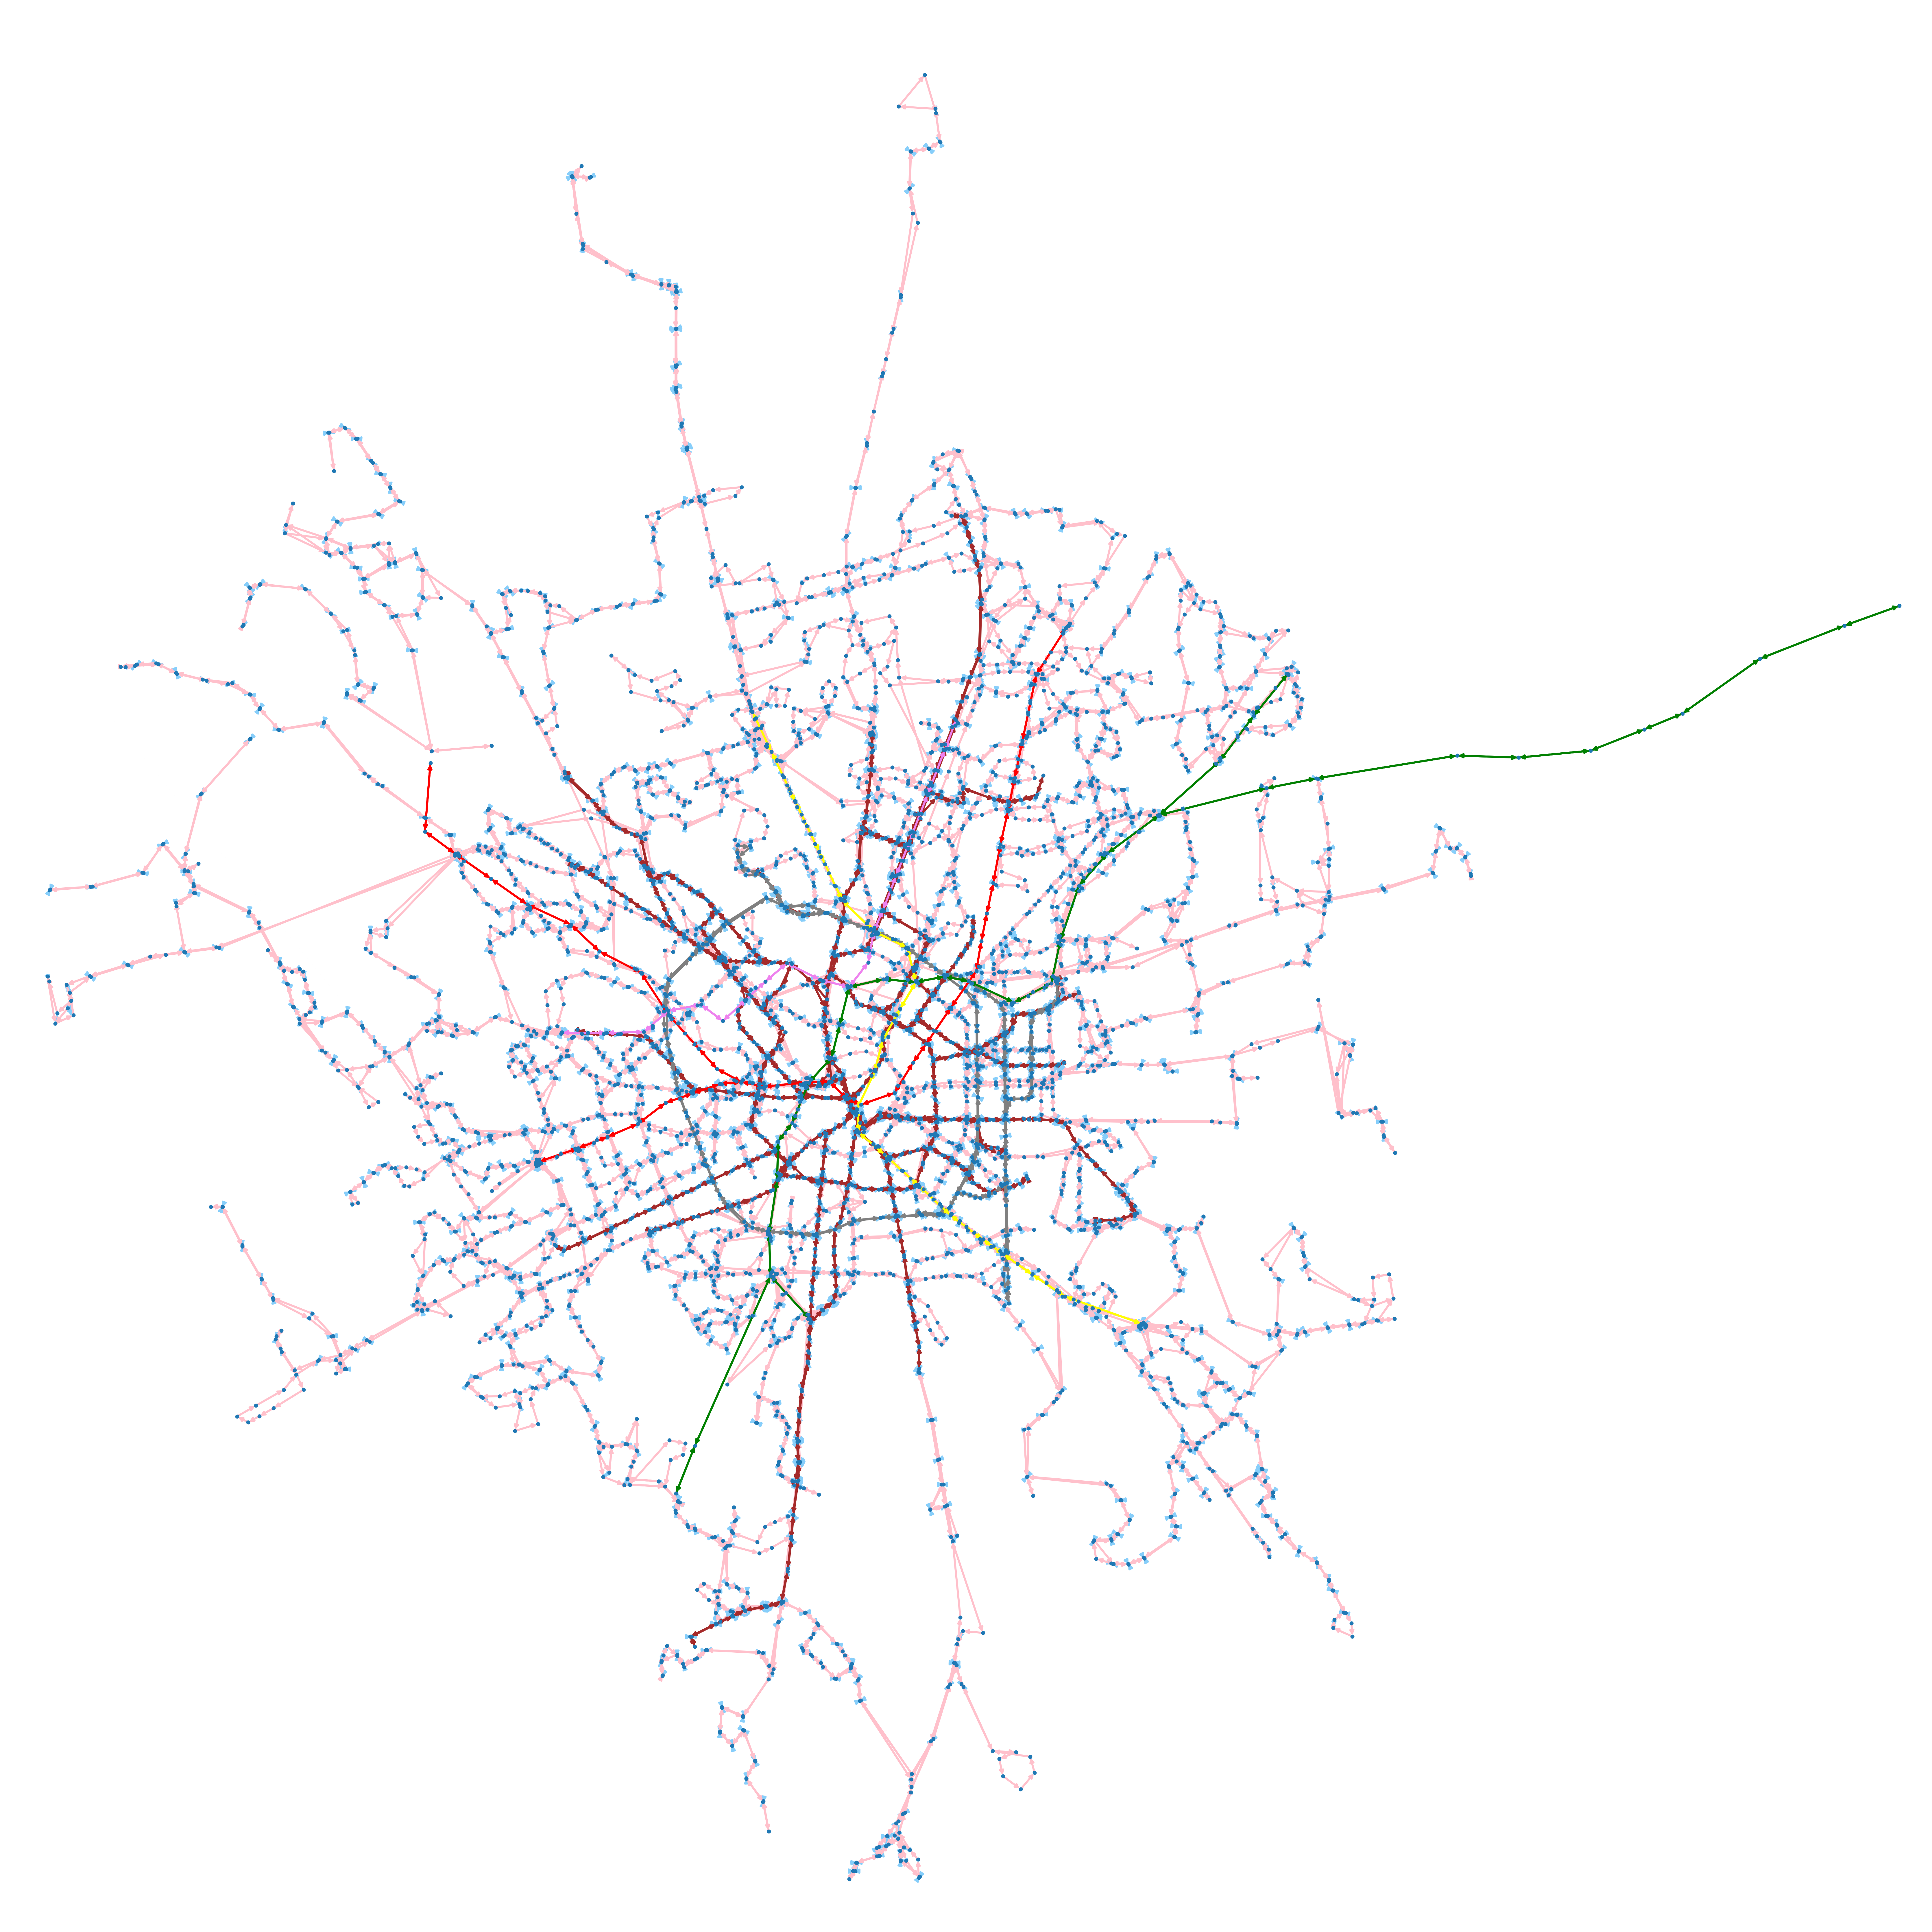
\includegraphics[scale = 0.5]{tex/pics/network_complete_cut.png}
    \caption{The public transportation network of Milan. Different transportation means are represented with different colors: metro line 1 is in rer, metro line 2 in green, metro line 3 in yellow, metro line 5 in violet, tram in brown, bus in pink and filobus in grey. Walking paths, for ($r_{foot} = 200 m$), are shown in light skyblue.}
    \label{network_complete}
\end{figure}

 \subsection{The Agents}\label{sec3}
 
Agents in the model represent the share of Milan's population which during weekdays move around the city using public transports. Each agent belongs to one among 4 possible age classes: 15-24, 25-44, 45-64 and over 65. They start their daily routine at home, perform 1 to 5 activities (among education, work, leisure, self-care/eating \footnote{ISTAT actually provides a category that includes eat, sleep and other self-care. However, given the time horizon we consider (5:00 a.m  to 1:00 a.m), we assume that “sleep” can be neglected.} and housework) and, eventually, go back home. Datasets from 8 to 10 are used to create a population which resembles the real population of residents in Milan.  \\
The creation of the synthetic population proceeds through different steps.
%  as summarised in the algorithm \ref{alg1} below.

First of all, for each agent we draw an age class from the distribution of inhabitants of Milan. Then, we draw a NIL for the agent's house from the distribution of the NILs conditional on the chosen age group \cite{site18}. After this, we draw uniformly at random, from the stops in the selected NIL, a precise node which represents the agent’s home. 

At this point, two possible strategies can be adopted to assign a travel diary to the agents:
\begin{itemize}
    \item \textbf{Strategy 1.} For each of the five possible activities we decide whether the agent will or not perform it during the day, by drawing from a Bernoulli with parameter equal to the probability that the agent carries it out such activity in an ordinary weekday, conditional on the agent's age class. Data used to construct this probability distribution come from dataset 9. Adopting this strategy, each agent can have a variable number of activities to carry out, ranging from 1 to 5.
    \item \textbf{Strategy 2.} Agents are forced to perform a number k of activities. The sequence of activities to perform is  drawn with replacement from the distribution of the combinations of activities conditional on the age group the agent belongs to. Specifically, we consider the choices of activities as independent from each other, so that the conditional probability of a combination of activities corresponds to the product of the conditional probabilities of the single activities..
\end{itemize}
In the original version of the model, strategy 1 has been adopted. We have realized that, on average, using stratey 1, around $20\%$ of the initially generated agents do not have any planned activity in their schedule and, therefore, we have decided to discard them. Experiments show that, on average, agents' schedule only contain 2 activities. To make the results of the two strategies comparable, the parameter k for the second strategy has been set to 2.

We assign a location to each activity selected for the agent (i.e., the specific node in the network) with probability proportional to the number of facilities corresponding to that task located nearby each node \cite{site9}. Among the possible categories proposed by OpenStreetMap, we only take into consideration the ones that match the ISTAT activities (eg. schools, universities, etc. for education; offices, co-working place, etc. for work; cinema, gyms, etc. for leisure time; restaurants, bars, etc. for eat/sleep). When the activity “housework” is selected, we assign as destination the agent’s house node. We then assign a departure time for each scheduled activity by drawing a 10-minutes time slot from the distribution of oriented movements over time conditional on the specific activity \cite{site11}, which has to be performed approximately 40 minutes after the departure (40 minutes being the average traveling time). To allow for minute-by-minute departure times, we also include a randomization term that adds or removes at most 5 minutes from the picked time. 

Finally, if the last destination of the agent is not “home”, we compute a critical time at which we let the agent depart again to go back home (time of the last activity + 40 min + average duration of last activity \cite{site11} + noise in the [-10 min, +10 min] interval). We consider two possible sets of average durations for the activities:
\begin{itemize}
\item set 1: 120 min for sleep/eat/personal care, 330 min for education, 440 min for paid work and 90 min for free time;
\item set 2: 120 min for sleep/eat/personal care, 156 min for education, 220 min for paid work and 90 min for free time.
\end{itemize}
The numbers in the first set have been computed by averaging across age-classes the duration of activities from ISTAT data. In set 2 the average duration of education and paid work have been reduced by 50\% as to allow for part-time occupations. 
The set used to compute the critical time is randomly chosen, for each agent, through a bernoulli draw with parameter $p_{long}$ equal to the probability of chosing set 1 (the one with longest average duration of activities). We set $p_{long}$ at 0.7 if the time of the last activities is before 1.30 a.m. and to 0.3 if it is after, as we believe that there is a higher chance of performing a long activity if that is started in the morning rather than in the second "half" of the day.
We assume that, if this critical time is after 10:30 p.m. the agent prefers not to use public transports to go back home, as the timetables are not favourable later in the evening.

\begin{algorithm}
\caption{Agents' generation}\label{alg1}
\begin{algorithmic}
\Require $n \geq 0$
\For {each agent $i = 1, ..., n$}:
\State \textit{age\_class} $\sim Multinomial(p_l)$ \Comment{$p_l$ = P(age class l) for $l = 1, ..., 4$}
\State $nil \sim Multinomial(q_{jl})$ \Comment{$q_j$ = P(nil j $\vert$ age\_class) for $j = 1, ..., 89$}
\State $home \sim Uniform(k)$ \Comment{$ k = \frac{1}{\vert \{s: s \in nil \} \vert }$}
\For {each activity a = 1, ..., 5}:
\State $ u \sim Bernoulli(f_a)$ \Comment{$f_a$ = P(a $\vert$ age\_class)}
\If{$u = 1$}:
    \State $destination \sim Multinomial(g_s)$ \\\Comment{$g_s = \frac{\text{\# amenities of type a close to node s}}{\text{total \# of amenities of type a}}$}
    \State \textit{departure\_time} $\sim Multinomial(r_t)$ \\\Comment{$r_t$ = P(travel time $\vert$ a) + U(-5, 5)}
\EndIf
\EndFor
\EndFor
\end{algorithmic}
\end{algorithm}

At this point, for each agent we have: a unique id, the age group, the starting point (node on the network) and a schedule of activities (from 1 to 5 activities, with the related destination and the time at which the agent has to start the journey to get there), as shown in the table \ref{tab1} below. 

\begin{table}[h]
\centering
\caption{Example of agent's generation}\label{tab1}%
\begin{tabular}{ll|lll}
\multicolumn{2}{c|}{The agent} & \multicolumn{3}{c}{The schedule} \\ 
\toprule
Features      & Data      & Activity & Destination & Departure time \\ 
\midrule
Unique id & 7548 & 1) Education & V.le Bligny, 19 & 7:30\\
Age & 15-24  &  2) Work	& Duomo M3 & 14:15\\
Starting point & Corvetto M3 & 3) Leisure & Moscova & 19:25\\
\bottomrule
\end{tabular}
\end{table}

The final step to complete the synthesis of the population is to assign to each agent the list of edges that form the shortest path to reach their destinations (Example in table \ref{tab2} below). Specifically, the shortest path is calculated through the Dijkstra algorithm, using as weight the traveling time of each edge. However, not all nodes are taken into account in this process. In fact, the shortest path is computed on the subgraph of the edges constituting the lines that are active in a limited time window around the departure time. In this way, the agent can only select routes that are available at the time of their departure. Lastly, since we are working on a multigraph, it may be the case that two stops are linked by two different means of transport with same speed. In this case, the agent includes in the shortest path the edges that minimize the number of changes of vehicles needed.


Agents are characterized by a state, which can take four possible values: busy, waiting, traveling and finished. Busy agents are those that are currently in one of the facilities and do not have to travel. Waiting agents are the ones that are waiting at a stop in order to get on a vehicle. Traveling agents are situated on edges and they are moving to their next destination. Finally, finished agents are those that have already completed all the journeys in their daily schedule.

\subsection{The Model}

Once the population of agents has been sinthesized, all agents are initialized to the busy status. We simulate 20 hours, from 5:00 a.m. to 1:00 a.m. of the next day, and let agents move on the network to reach all the destinations in their schedule. 

Each iteration of the simulation represents one minute. At each minute, we activate agents within groups in random order, to avoid always giving the first-mover advantage to the same individual. We first consider the set of “busy” agents: if they are scheduled to depart at the current minute, their status changes to “waiting”, otherwise, they remain “busy” at their current position. We then loop over the “traveling” agents: looking at their path, they evaluate whether they have to get off the current vehicle and disembark if that is the case. Clearly, they can only do so if the vehicle has crossed the edge and reached the next stop. Edges in the graph can be either active or inactive at any given time step: an edge is active at minute t if there’s a vehicle that is passing at the starting node of the edge and can embark passengers. “Waiting” agents are the last to act: each of them looks at the next edge in their path and, if it is active and there’s space on the vehicle, they get on board, while, if that is not the case, they stay on the stop waiting for the next activation. Once an angent completes all of their tasks, their status changes to “finished” and they are no longer considered in the following iterations. It can happen that agents are scheduled to depart for an activity very late in the night, when rides are less frequent, so they fail to complete their journey, and their status never becomes “finished”. We assume that they will use alternative ways, not covered in our model, to proceed.

The model's structure can be summarized by mapping its elements into the sets presented in Borgonovo (2022) [INSERISCI LA CITAZIONE]:
\begin{itemize}
\item Principles: A principle of the model is that agents' houses are exactly on transport lines' stops: indeed, the environment in this model is not the continuous space of the area of Milan, but only the points representing stops and the lines connecting them. We believe this simplification is reasonable, as we assume that the path from agents' houses to the closest stop is negligible (there is no path, using public transportation, allowing agents to reach the closest stop to their location, as it is the closest). Hence, we assume the departure times are not the times at which the agents plan to live their houses (or, more in general, their location) but the times at which they will be at the stop, ready to enbark on a vehicle. Another principle of the model is the characterization of agents through a status taking 4 possible values: busy, waiting, traveling and finished. A status characterizes the behaviour of an agent in future steps. We believe that making changes to the statuses system, for example as to allow for other values for agents' status, would lead to a different model. 
\item Assumptions: An assumption of the model is that agents move on the environment represented by the network of public transports of the city of Milan and have full knowledge of the network, so that they are able to plan in advance the path to follow in order to minimize traveling time. The current version of the network is built on data updated to 05/05/2022. Any update to the routes would result in a different version of the network, but that would not change the essence of the model. Agents, however, are not available of lines' timetables: they assume that the vehicles will be immediately available at the stop when they arrive, and they are willing to wait for it, as they believe that such vehicle is their best option.
\item Parameters linked to the environment: Two important parameters of the environment are the capacity and speeds of vehicles, that determine the weights of edges and, hence, the expected traveling time agents consider when deciding which path to follow. Another important parameter is the maximum distance used to consider two stops as "at walking distance" ($r_{foot}$). This is crucial as it dictates the number of fictitious "foot" edges added to the original network and, consequently, the total number of possible paths available. Finally, another parameter is the radius $r_{pois}$ of the ball centered at each stop, which we use to compute the number of points of interests that are reachable from each stop. This parameter plays an important role as it changes the probabilities of each activity being performed in proximity of any stop.
\item Agents' Parameters: The number of age classes and of possible activities the agents can perform are important parameters characterizing the agents' profiles. The distributions of age classes and of NILs given age classes are multinomial distributions whose parameters can be considered agents' parameters. Moreover, the probability of agents performing "long" tasks rather than short ones $p_{long}$ is an important parameter which influences agents' decision to return back home with public transports at the end of their schedule.
\item Procedures: Some procedures describe the way in which agents are able to enbark vehicles: first traveling agents get off, then waiting agents try to get on in random order, succeeding unless full capacity of the vehicle is reached. Another interesting procedure is the strategy used to sample activities: the standard one is to allow for one possible occurrence of each activity during the day; an alternative is to allow for repetitions up to a number k of total activities. 
\end{itemize}